\documentclass[12pt]{article}
\usepackage[margin=1.0 in]{geometry}
\addtolength{\topmargin}{.25in}
\usepackage[utf8x]{inputenc}  
\usepackage{amsmath}
\usepackage{calc}
\usepackage{array}
\usepackage{amssymb}
\usepackage{tikz}
\usepackage{pgfgantt}
\usepackage{hyperref}
\usepackage{graphicx}
\usepackage{upquote}
\newcommand{\HRule}{\rule{\linewidth}{0.5mm}}
\usepackage{hyperref}
\newcommand{\Green}{\tikz\draw[green,fill=green] (0,0) circle (1 ex);}
\newcommand{\Lime }{\tikz\draw[brown,fill=brown] (0,0) circle (1 ex);}
\newcommand{\Blue}{\tikz\draw[blue,fill=blue] (0,0) circle (1 ex);}
\newcommand{\Yellow}{\tikz\draw[yellow,fill=yellow] (0,0) circle (1 ex);}
\newcommand{\Red}{\tikz\draw[red,fill=red] (0,0) circle (1 ex);}
\renewcommand*\contentsname{Indholdsfortegnelse}
\definecolor{listinggray}{gray}{0.9}
\usepackage{listings}
\lstset{
	language=,
	literate=
		{æ}{{\ae}}1
		{ø}{{\o}}1
		{å}{{\aa}}1
		{Æ}{{\AE}}1
		{Ø}{{\O}}1
		{Å}{{\AA}}1,
	backgroundcolor=\color{listinggray},
	tabsize=3,
	rulecolor=,
	basicstyle=\scriptsize,
	upquote=true,
	aboveskip={1.5\baselineskip},
	columns=fixed,
	showstringspaces=false,
	extendedchars=true,
	breaklines=true,
	prebreak =\raisebox{0ex}[0ex][0ex]{\ensuremath{\hookleftarrow}},
	frame=single,
	showtabs=false,
	showspaces=false,
	showstringspaces=false,
	identifierstyle=\ttfamily,
	keywordstyle=\color[rgb]{0,0,1},
	commentstyle=\color[rgb]{0.133,0.545,0.133},
	stringstyle=\color[rgb]{0.627,0.126,0.941},
}
\begin{document}
\begin{titlepage}
\begin{center}

\textsc{\Large Bachelor Thesis \\ Optimized pattern matching in genomic data\\[0.3cm]}
\HRule \\[0.4cm]
{ \LARGE \bfseries Synopsis}\\[0.4cm]
\HRule \\[1.2cm]
\textsc{\large Martin Westh Petersen - mqt967 \\ Kasper Myrtue - vkl275}\\[1.0cm]
\end{center}
\begin{center}
\vfill
{\large 23. Februar 2015}
\end{center}
\end{titlepage}
\section{Problem definition}
Is it possible to re-implement/modify scan\_for\_mathces, so that it has an equal or
increased performance? \\ \\
As a minimum, our product will contain the following features:
\begin{itemize}
\item Constructing literal pattern units (e.g. "AGUUG") that are used for finding a specific sub-sequence in the 
database sequence.
\item Allowing for wildcards (e.g. "AGWUUG" where "W" matches multiple other bases).
\item Allowing any pattern unit a specified number of insertions, deletion and mismatches (e.g. "AGGUAAA[2,0,3]").
\end{itemize}
In order for our program to meet in the minimum requirements for the users, the following core features will also be needed.
If time allows, as many as possible will be implemented as well.
\begin{itemize}
\item Constructing ambiguous pattern units (e.g. "4..8") that match any sub-sequence with a possibility for a 
flexible range.
\item Combining pattern units to a full pattern that defines the full search criteria when scanning the database sequence.
\item Defining variables for referencing pattern units (e.g. "p1=5..6") that can be used 
to find related patterns that are unknown before search (e.g. p1=5..6 p1[1,0,0])
\item The $\sim$ symbol can be inserted in front of any pattern unit to indicate that we are looking for the reversed
complement of that pattern unit.
\item A more optimized way of searching for matches, given
complex patterns consisting of multiple pattern units. E.g. the order of which the different pattern units are searched
can be optimized to increase performance instead of going through the pattern units from one end to the other. 
\end{itemize}
\section{Limitations}
In case of excess time, secondary features may be implemented: 
\begin{itemize}
\item Is it possible to optimize the backtracking algorithm for string search, so that the order of the possibilities 
tried regarding insertions, deletion and mismatches results in a conclusion faster.
\item Logical "or" between patterns (e.g. "(AUUG $|$ AGGG)") that matches either of the sub-sequences.
\item A possibility for defining custom "pairing rules" (e.g. "r1={au,ua,gc,cg,ga,ag}") that can be used for 
for defining allowances when comparing a reversed complement pattern unit (e.g. "r1$\sim$p1").
\item An analysis of the complexity and running time of the program.
\end{itemize}
Every feature from scan\_for\_mathces beyond what has been mentioned will not be implemented.
\section{Motive}
Pattern matching functionality for strings in genomic data is very useful, 
but requires a good performance due to huge amounts of data. 
Scan\_for\_matches serves this purpose, but big improvements in performance can be made.
On top that, the code is poorly documented, lacks version control and the code is hard to read and maintain.
\section{Tasks and schedule}
Below is a list of the tasks that this project consists of:
\begin{itemize}
\item \textbf{Research} 
\begin{enumerate}
\item Why is scan\_for\_matches fast despite the use of a backtracking algorithm? This research task is about 
reading and understanding the vital parts of the scan\_for\_matches code so that we understand the overall
ideas and algorithms, and can reuse them if needed.
\item How should the interface be improved to best suit the users? E.g. Should the program be started and
patterns specified in a command-line manner or reading of files? How should the output be displayed or stored?
\item What functionality should we be focused on implementing. This task ensures that the most important functionality is 
identified, so a proper prioritization can be made. This task is already completed and the result is shown as the list
of primary features and the list of secondary features.
\item Researching what methods and algorithms for string-handling that exists, and exploring different options for 
choosing a programming language to work with.
\end{enumerate}
\item \textbf{Analysis}
\begin{enumerate}
\item Choosing a language for implementation. (It will probably be C or C++).
\item Figuring out the overall methods and algorithms that we are going the use.
\item Deciding on how the user interface should work, e.g. how will patterns, input and output be provided, displayed 
and/or stored.
\end{enumerate}
\item \textbf{Design}
\begin{enumerate}
\item Designing the overall structure of the program.
\end{enumerate}
\item \textbf{Implementation}
\begin{enumerate}
\item First prototype that can search the database sequence for a single literal pattern unit and provide the output.
\item Second prototype allows ambiguous patterns with flexible length, and the possibility of combining pattern units
into one single pattern.
\item Third prototype includes all the 6 core functions defined earlier.
\item The fourth prototype will include the optimized order of searching for the different pattern units.
\end{enumerate}
\item \textbf{Testing}
\begin{enumerate}
\item A thorough test of our implementation on the given data to verify that each of the implemented features work
\item Testing the running time of both simple and complex patterns with the original scan\_for\_matches against our
implementation.
\end{enumerate}
\item \textbf{Documentation} - The documentation will start being written when we start the implementation period
and finish before final report is due. It will consist of the comments written in the code and a user guide provided 
together with the program.
\item \textbf{Report}
\begin{enumerate}
\item Midway report
\item Final report
\end{enumerate}
\end{itemize}
Figure 1 shows our schedule for the project, with the the implementation period consisting of the 4 different milestone
prototypes of the program. The midway report and final report is shown as dots in the bottom.
\begin{figure}[h!]
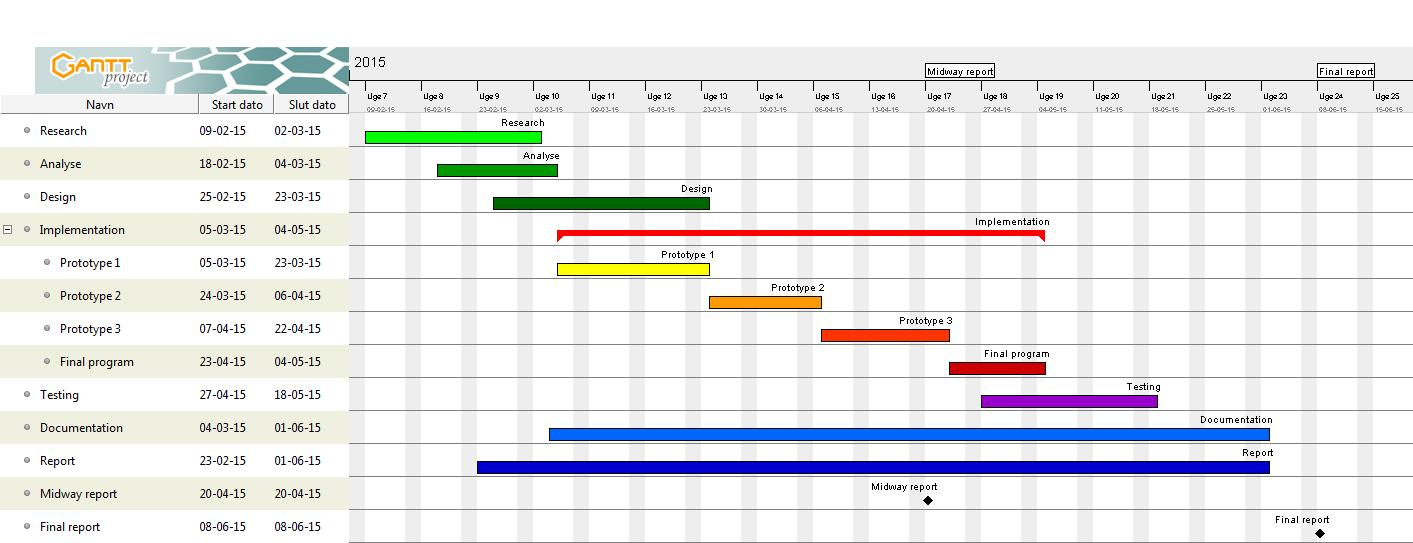
\includegraphics[scale=0.7]{gantt.png}
\caption{Schedule}
\end{figure}

\end{document}
